% ------------------------------------------------------------------------------
% TYPO3 Version 10 LTS - What's New (French Version)
%
% @license	Creative Commons BY-NC-SA 3.0
% @link		https://typo3.org/help/documentation/whats-new/
% @language	French
% ------------------------------------------------------------------------------

\section{Introduction}
\begin{frame}[fragile]
	\frametitle{Introduction}

	\begin{center}\huge{\color{typo3darkgrey}\textbf{Introduction}}\end{center}
	\begin{center}\large{\textit{Faits et chiffres clés de TYPO3 v10 LTS}}\end{center}

\end{frame}

% ------------------------------------------------------------------------------
% TYPO3 Version 10 LTS - The Facts

\begin{frame}[fragile]
	\frametitle{Introduction}
	\framesubtitle{TYPO3 Version 10 LTS}

	\begin{itemize}
		\item Date de sortie~: 21 avril 2020
		\item Type de sortie~: LTS (Support à long-terme)
	\end{itemize}

	\begin{figure}
		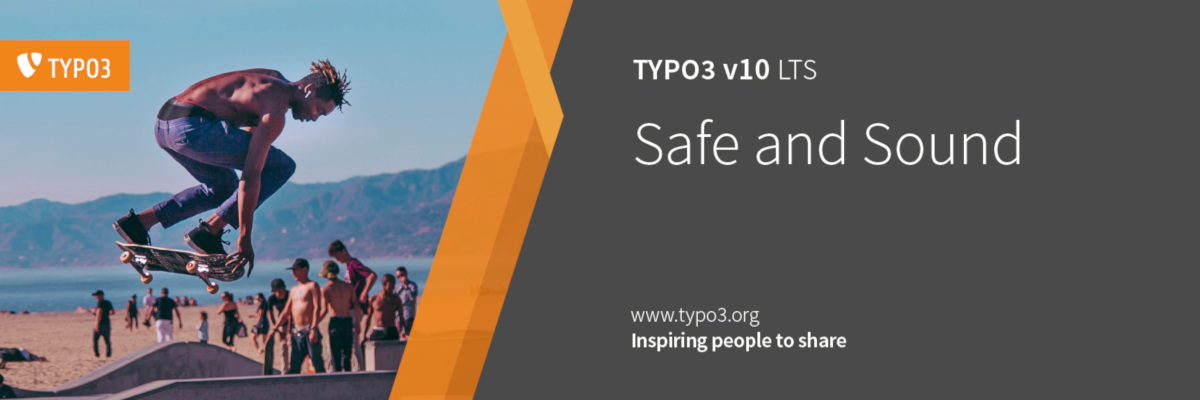
\includegraphics[width=0.95\linewidth]{Introduction/typo3-v10-4-banner.jpg}
	\end{figure}

\end{frame}

% ------------------------------------------------------------------------------
% TYPO3 Version 10 LTS - Executive Summary

\begin{frame}[fragile]
	\frametitle{Introduction}
	\framesubtitle{En Résumé}

	\small
		TYPO3 v10.4 (aussi appelé TYPO3 v10 LTS indiquant que c'est la version de support à long-terme)
		est notre nouvelle version phare et est, sans conteste, l'un des systèmes de gestion
		de contenu open-source en PHP les plus avancés du marché à date.

		\vspace{0.2cm}

		Après la publication de cinq itérations depuis juillet 2019, nous pouvons fièrement
		affirmer que nous avec équipé TYPO3 avec les dernières bibliothèques PHP modernes et
		que nous avons introduit de nouvelles fonctionnalités fantastiques pour les entreprises.

		\vspace{0.2cm}

		Ce document résume les changements les plus importants entre TYPO3 v9 LTS et v10 LTS
		d'un point de vue technique.

%		\vspace{0.2cm}
%
%		"What's New Slides" of all TYPO3 v10.x releases are available at
%		\href{https://typo3.org/help/documentation/whats-new/}{typo3.org}.

% changelog
% what's new slides

	\normalsize

\end{frame}

% ------------------------------------------------------------------------------
% System Requirements

\begin{frame}[fragile]
	\frametitle{Introduction}
	\framesubtitle{Configuration requise}

	\begin{itemize}
		\item Version 7.2, 7.3 ou 7.4 de PHP
		\item Configuration PHP~:

			\begin{itemize}
				\item \texttt{memory\_limit} >= 256M
				\item \texttt{max\_execution\_time} >= 240s
				\item \texttt{max\_input\_vars} >= 1500
				\item L'option de compilation \texttt{-}\texttt{-disable-ipv6}
					\underline(NE) doit \underline{PAS} être utilisée
			\end{itemize}

			\item Extensions PHP requises~:\newline
				\small
					filter, hash, openssl, pcre >= 8.38, session, SPL, standard,
					xml, zip and zlib
				\normalsize

		\end{itemize}

\end{frame}

% ------------------------------------------------------------------------------
% System Requirements

\begin{frame}[fragile]
	\frametitle{Introduction}
	\framesubtitle{Prérequis système}

	\begin{itemize}
		\item Serveur web tel qu'Apache, Nginx, IIS, etc.
		\item Tout moteur de base de données pris en charge par \textbf{Doctrine DBAL}.
			Par exemple~:
	\end{itemize}

	\begin{figure}
		
\includegraphics[width=0.70\linewidth]{Introduction/logo-databases.png}
	\end{figure}

	\begin{itemize}
		\item Espace disque minimum nécessaire~: 200~Mo
		\item Le backend prend en charge tous les navigateurs modernes comme Microsoft Edge,
			Google Chrome, Firefox, Safari ou compatibles.
	\end{itemize}

\end{frame}

% ------------------------------------------------------------------------------
% Sprint Releases

\begin{frame}[fragile]
	\frametitle{Introduction}
	\framesubtitle{Chronologie des développements}

	Itérations publiées~:
	\vspace{0.4cm}
	\begin{itemize}
		\item v10.0 \tabto{1.1cm}23/Jui./2019\tabto{3.4cm}Ouvre la voie à de nouveaux concepts et APis
		\item v10.1 \tabto{1.1cm}01/Oct./2019\tabto{3.4cm}Améliorations routage et gestion des sites V2
		\item v10.2 \tabto{1.1cm}03/Déc./2019\tabto{3.4cm}Améliorations du moteur de rendu Fluid
		\item v10.3 \tabto{1.1cm}25/Fév./2020\tabto{3.4cm}Gèle des fonctionnalités
		\item v10.4 \tabto{1.1cm}21/Avr./2020\tabto{3.4cm}Version LTS (Long-term Support)
	\end{itemize}

\end{frame}

% ------------------------------------------------------------------------------
% LTS Support Timeline

\begin{frame}[fragile]
	\frametitle{Introduction}
	\framesubtitle{Support à long-terme}

	\begin{figure}
		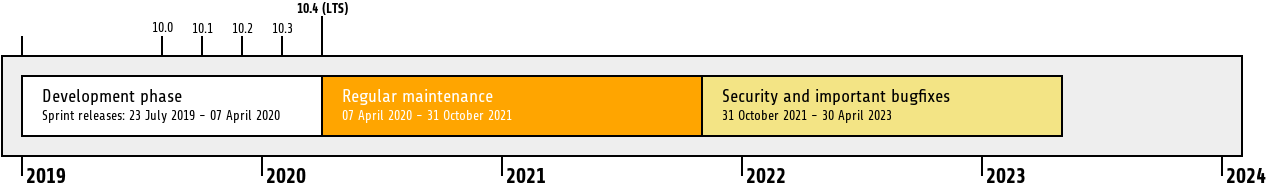
\includegraphics[width=1\linewidth]{Introduction/typo3-v10-lifecycle.png}
	\end{figure}

	\begin{itemize}
		\item La version 10.4 de TYPO3 est version LTS (support à long-terme)
		\item Maintenance régulière et corrections jusqu'en octobre 2021
		\item Corrections critiques et de sécurité jusqu'en avril 2023
	\end{itemize}
	\vspace{0.2cm}
	\textbf{Support étendu}\newline
	\smaller
		\href{https://typo3.com}{TYPO3 GmbH} fournit le support à long-terme étendu
			(ELTS) pour TYPO3 v10 LTS jusqu'en avril 2026.
	\normalsize

\end{frame}

% ------------------------------------------------------------------------------
